\documentclass[a4paper,11pt]{article}
\usepackage[utf8]{inputenc}
\usepackage[spanish]{babel}
\usepackage{graphicx}
\begin{document}
\title{Proyecto Final}
\author{Pedro Alcoba Gómez et al.}
\date{15/10/2018}
\begin{abstract}
	Este es el proyecto final del curso de Git y \LaTeX{} aplicado a la investigación científica.
	\\\\
	https://github.com/pedralcg/proyecto\_final/
	\\
\textbf{Palabras clave:} Pedro Alcoba, \LaTeX{}, GitHub, Darwin Eventur  
\end{abstract}
\tableofcontents
\maketitle

\part{Introducción}
Hola, esto es una prueba del documento requerido para la práctica del ejercicio final del curso de Git y \LaTeX{} aplicado a la investigación científica.
\begin{figure}[h]
	\centering
		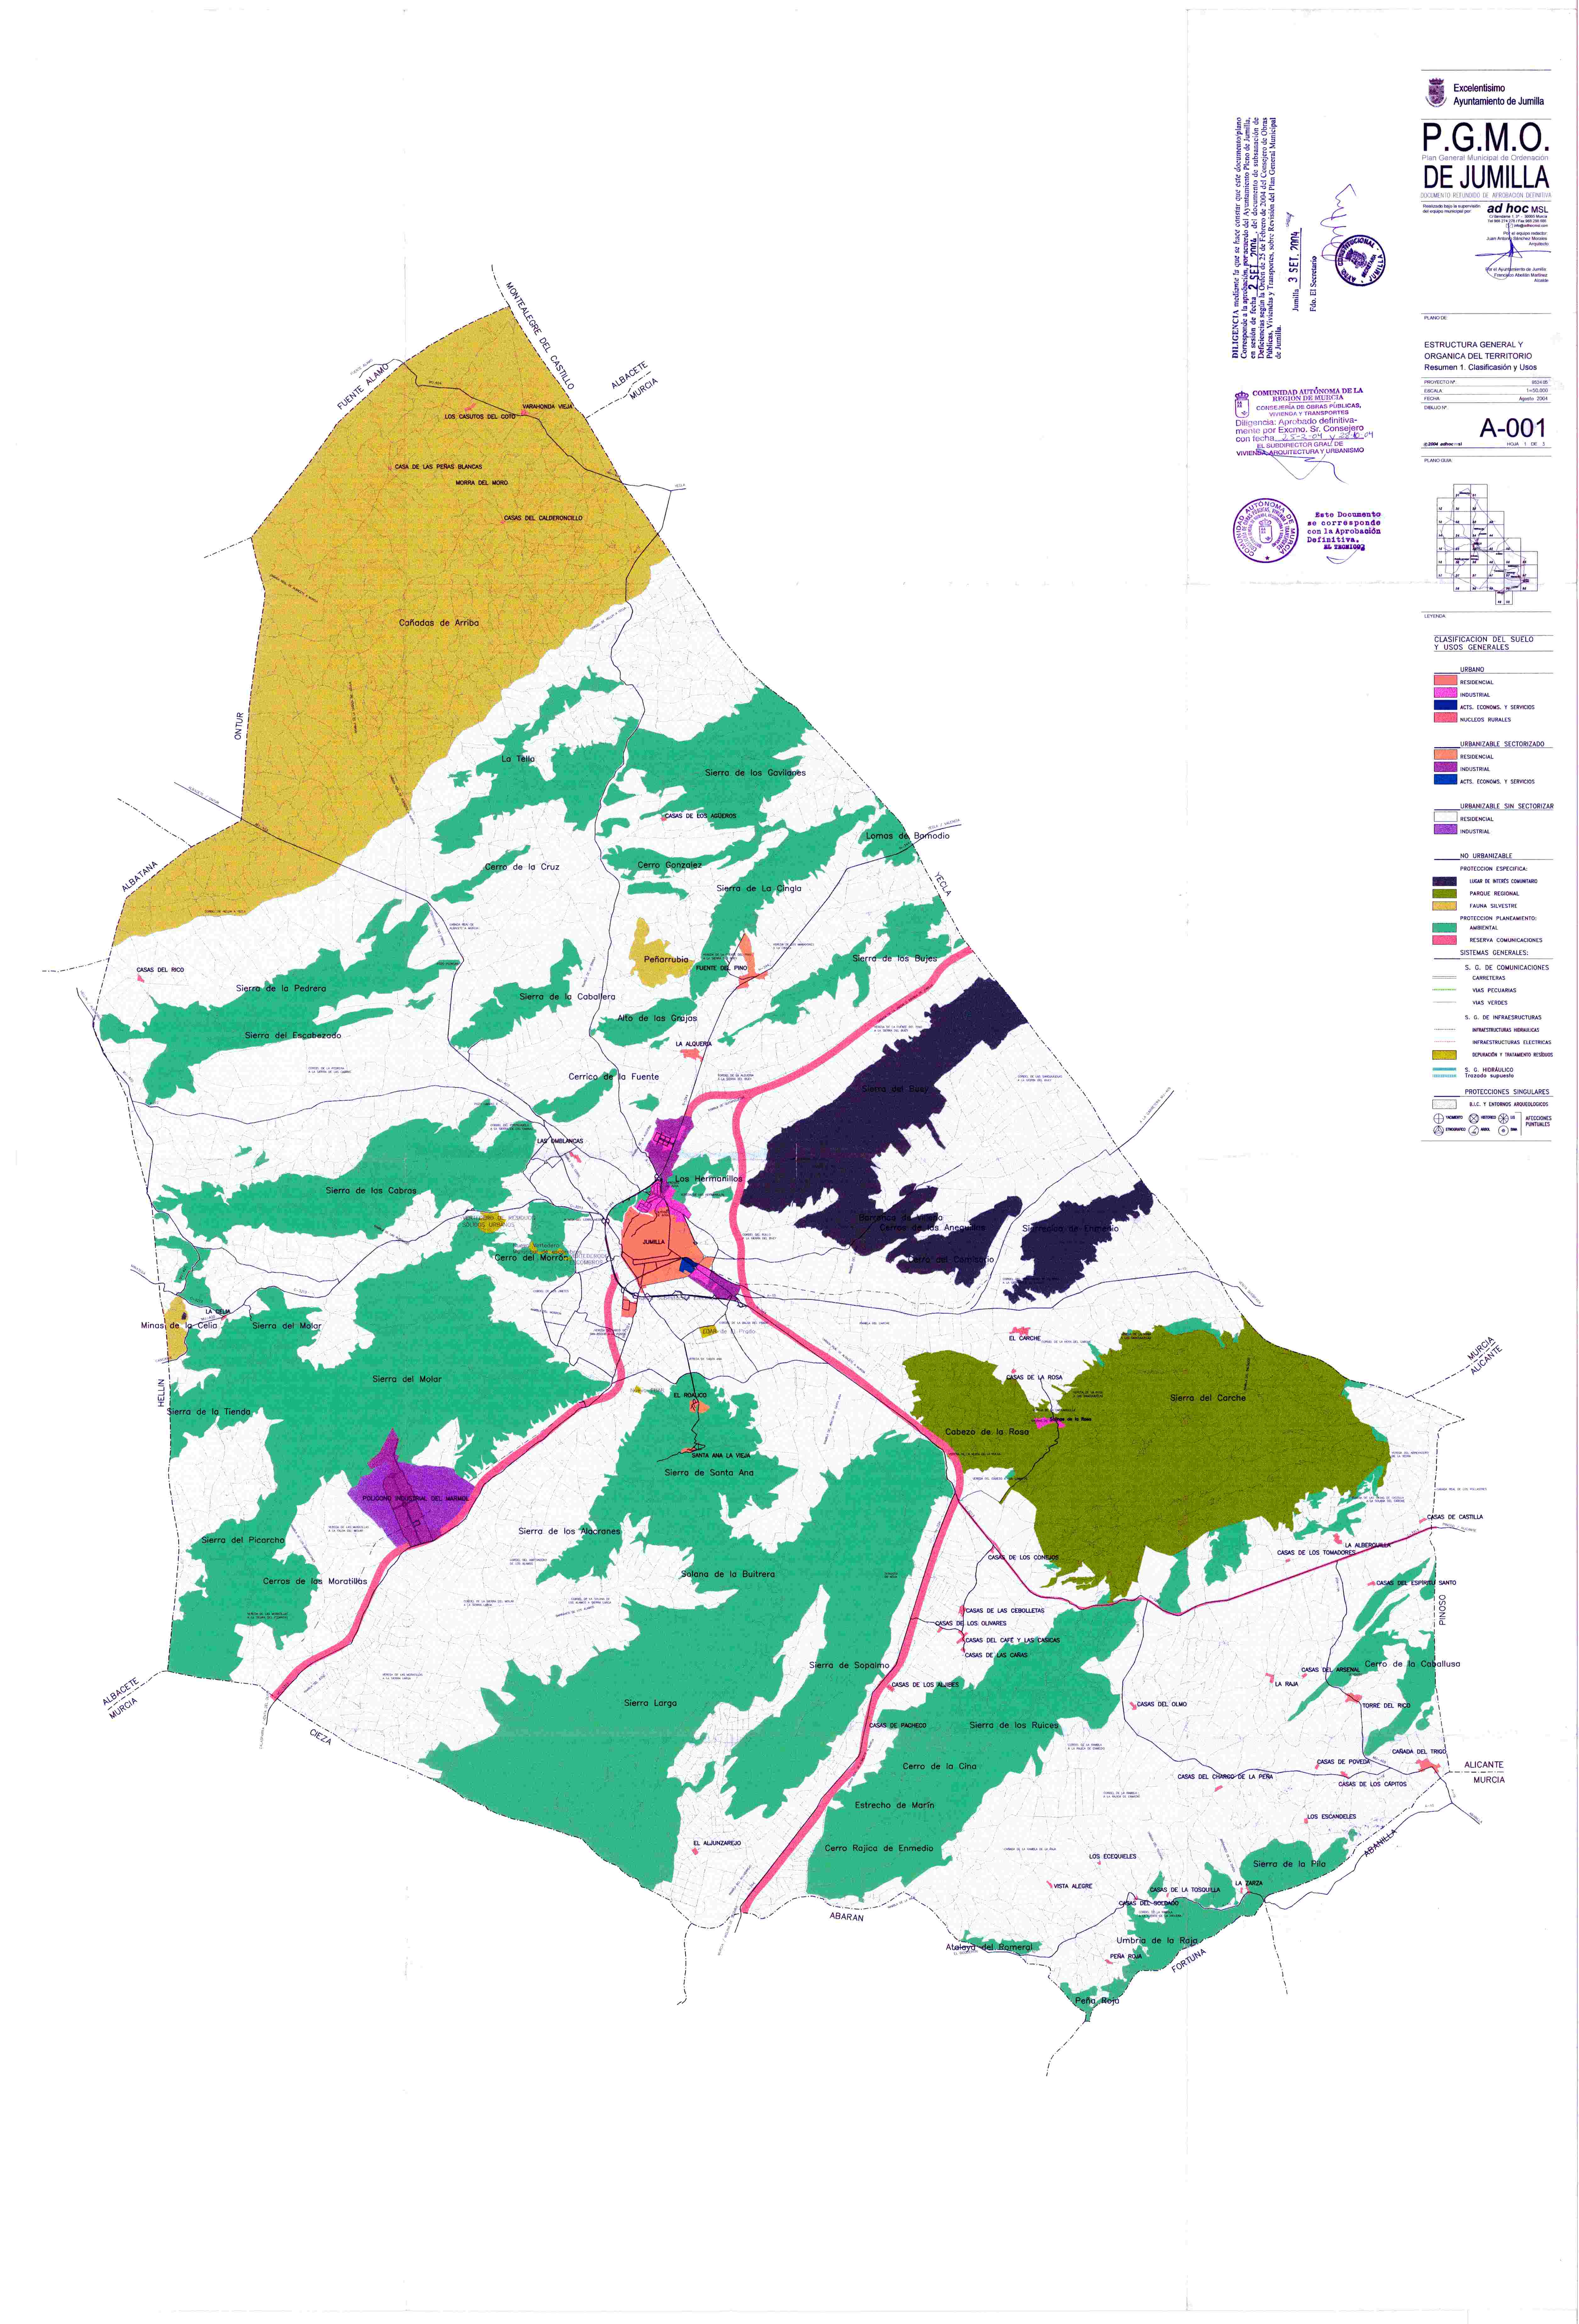
\includegraphics[width=150mm,height=100mm]{figura}
	\caption{PGMO Jumilla}
	\label{Figura}
\end{figure}

Lorem ipsum \cite{Bib01}dolor sit amet, consectetur adipiscing elit. Sed mollis id arcu sit amet scelerisque. Praesent vehicula nulla et mauris convallis, ultricies rhoncus nulla bibendum. Proin nunc leo, dapibus in porttitor vitae, malesuada sed tellus. Mauris eget facilisis mi, ut eleifend dui. Aliquam erat volutpat. Nulla ut eros dui. Suspendisse potenti. Donec quis eros non enim egestas lobortis in quis risus. Donec mattis ultricies commodo. Proin feugiat lacus nunc, id euismod sapien aliquet et. Proin pulvinar placerat congue. Proin nisl sem, eleifend eu sagittis tempus, hendrerit ac ligula. Suspendisse porttitor elit in posuere cursus. Quisque in elit molestie, elementum est sed, iaculis sem. Orci varius natoque penatibus et magnis dis parturient montes, nascetur ridiculus mus.

Cras iaculis elit et rhoncus porttitor. Nulla facilisi. Etiam interdum mattis ante nec sodales. Donec eros erat, viverra vel feugiat vitae, pharetra ut massa. Vestibulum quis auctor justo. Morbi placerat efficitur tortor id vestibulum. Morbi quis turpis velit. Cras non posuere metus, eget suscipit nunc. Nam urna urna, vulputate sed eleifend in, tincidunt eu sem. Maecenas id consequat velit. Aenean massa massa, fringilla et sollicitudin ut, iaculis id lacus.

Nulla nibh tellus, pharetra ut molestie sed, dignissim a lacus. Proin sed rutrum massa. Vestibulum eleifend aliquam convallis. Suspendisse fringilla iaculis massa. Interdum et malesuada fames ac ante ipsum primis in faucibus. Suspendisse fringilla lorem in massa laoreet, sed mollis ipsum sagittis. Sed ultrices est at est fermentum aliquet. Class aptent taciti sociosqu ad litora torquent per conubia nostra, per inceptos himenaeos. Morbi varius auctor purus, placerat ullamcorper orci efficitur eu. Aenean id tristique urna. Etiam iaculis turpis eu diam venenatis convallis.\\\\

\begin{table}[htb]
	\begin{center}
		\begin{tabular}{|l|l|l|}
			\hline
			Banda & Resolución espacial & Longitud de onda (mm) \\
			\hline \hline
			2 & 10 m & 490 \\ \hline
			3 & 10 m & 560 \\ \hline
			5 & 20 m & 705 \\ \hline
			9 & 30 m & 945 \\ \hline
			11 & 20 m & 1610 \\ \hline
		\end{tabular}
		\caption{Bandas del satélite Sentinel 2}
	\end{center}
\end{table}

Quisque suscipit id risus vel sollicitudin. Duis eget turpis imperdiet, fermentum ante tempor, facilisis nisl. Aliquam magna dui, eleifend sit amet pellentesque a, lobortis id sapien. Phasellus tristique suscipit mi quis rutrum. Pellentesque elit purus, malesuada eget risus vitae, volutpat ullamcorper mauris. Interdum et malesuada fames ac ante ipsum primis in faucibus. Mauris egestas sed quam sed lacinia. Vivamus pellentesque justo velit, ut efficitur felis dignissim tincidunt. Nulla eros mauris, scelerisque a mollis et, vehicula ac dui.

Aenean enim lectus, bibendum sed nisl nec, cursus porttitor justo. Donec in augue nibh. Fusce aliquam massa at tellus porttitor, nec lacinia nisl tempor. Etiam tincidunt rutrum odio eu aliquam. Integer leo diam, volutpat sed nisi commodo, faucibus luctus sapien. Integer aliquam laoreet est, a pulvinar diam mollis sit amet. Nam erat erat, faucibus a dolor vel, vulputate varius tortor. Donec elit diam, malesuada non tempus a, vulputate sed purus. In hac habitasse platea dictumst. Vivamus blandit tortor hendrerit augue aliquam interdum. Praesent dui ligula, lacinia sit amet nisl nec, mollis condimentum dolor. Vivamus elementum lacus quis mi consectetur fringilla.

\part{Estado del arte}

Lorem ipsum dolor sit amet, consectetur adipiscing elit. Nam eleifend mi ut augue pellentesque, at pellentesque mauris vehicula. Sed dignissim non dui id suscipit. Duis mollis vestibulum nibh, sed iaculis risus faucibus sit amet. Sed lectus orci, porta vitae mi sed, tincidunt semper diam. Donec porttitor varius convallis. Lorem ipsum dolor sit amet, consectetur adipiscing elit. Integer in felis convallis, laoreet massa ut, imperdiet justo. Etiam mollis aliquet nisl in imperdiet. Morbi semper ex tortor, non luctus arcu semper nec. Sed vulputate consectetur dolor hendrerit mollis. Aenean sed placerat libero. Mauris vitae nibh sed ante venenatis mollis. Sed arcu tortor, cursus sed ligula vitae, auctor fringilla ex. Nulla convallis eu eros sed vehicula. Quisque eu nulla in augue pretium commodo. Donec efficitur sed quam eu iaculis.

\begin{figure}[h]
	\centering
	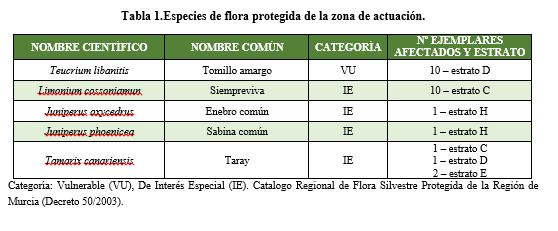
\includegraphics[width=100mm,height=50mm]{figura2}
	\caption{Tabla de especies protegidas}
	\label{Figura}
\end{figure}

Integer molestie euismod ex, quis facilisis nibh semper sed. Morbi lacinia sit amet sem at vestibulum. Nullam magna nisl, euismod sollicitudin dictum malesuada, fermentum at dolor. Ut sed molestie mauris, vel tempus risus. Donec mattis, nisi in sagittis pretium, ligula nunc ultricies tellus, id interdum lacus dolor in magna. Suspendisse in dui tincidunt, tempor ipsum a, suscipit urna. Donec eu libero sollicitudin ipsum mattis pulvinar. Nullam magna sem, iaculis sit amet nisi a, dictum interdum neque. Donec justo diam, elementum non volutpat ut, fermentum vitae odio. Suspendisse scelerisque ex odio, eget semper est pharetra tempor. Nam sit amet augue risus. Nunc erat lacus, congue eu magna in, hendrerit auctor ex. Aenean ullamcorper vitae nunc eu sagittis.

Suspendisse mauris arcu, bibendum ut nisi vitae, eleifend efficitur lectus. Morbi porta justo eu aliquam placerat. Maecenas ante tellus, semper condimentum nisi eget, ultrices consectetur mauris. Maecenas interdum efficitur ante eget malesuada. Duis hendrerit porta erat ut pretium. Aenean quis viverra metus. Vivamus vestibulum commodo sapien sit amet egestas. Sed ut velit sed sem commodo mattis. Vivamus aliquam, ante eu tincidunt pulvinar, tellus nisl vehicula dui, non pellentesque odio eros a ipsum. Donec elementum nec sapien a dignissim. Sed interdum ligula leo, at bibendum elit pellentesque nec. Phasellus egestas pulvinar ante. Quisque consequat a est eu gravida. Nullam tristique eleifend blandit.

Nullam eleifend commodo ipsum id convallis. Morbi suscipit, dui nec maximus aliquet, urna sem lacinia est, in luctus enim purus id velit. Aliquam tincidunt nisi eu metus condimentum ultricies. Quisque auctor leo eu libero ultricies, maximus dapibus nisl auctor. Quisque venenatis risus metus, nec ornare tortor dignissim cursus. Aenean volutpat viverra mollis. Vestibulum non condimentum turpis, non eleifend erat. Quisque pellentesque commodo turpis. Sed ut nulla egestas, convallis libero a, sodales ante. Aliquam tempor erat libero, vel facilisis nisl commodo in. Aliquam ornare lacus non egestas efficitur. Mauris a sapien eu magna ultrices pellentesque vitae et lacus. Donec maximus sit amet leo sit amet vestibulum. Nam non iaculis sapien, tempor sollicitudin nunc. Quisque dictum, lorem ac sagittis viverra, dolor erat euismod erat, vel lacinia magna lectus ut sapien. Integer volutpat libero feugiat lacus laoreet pulvinar.

\begin{figure}[h]
	\centering
	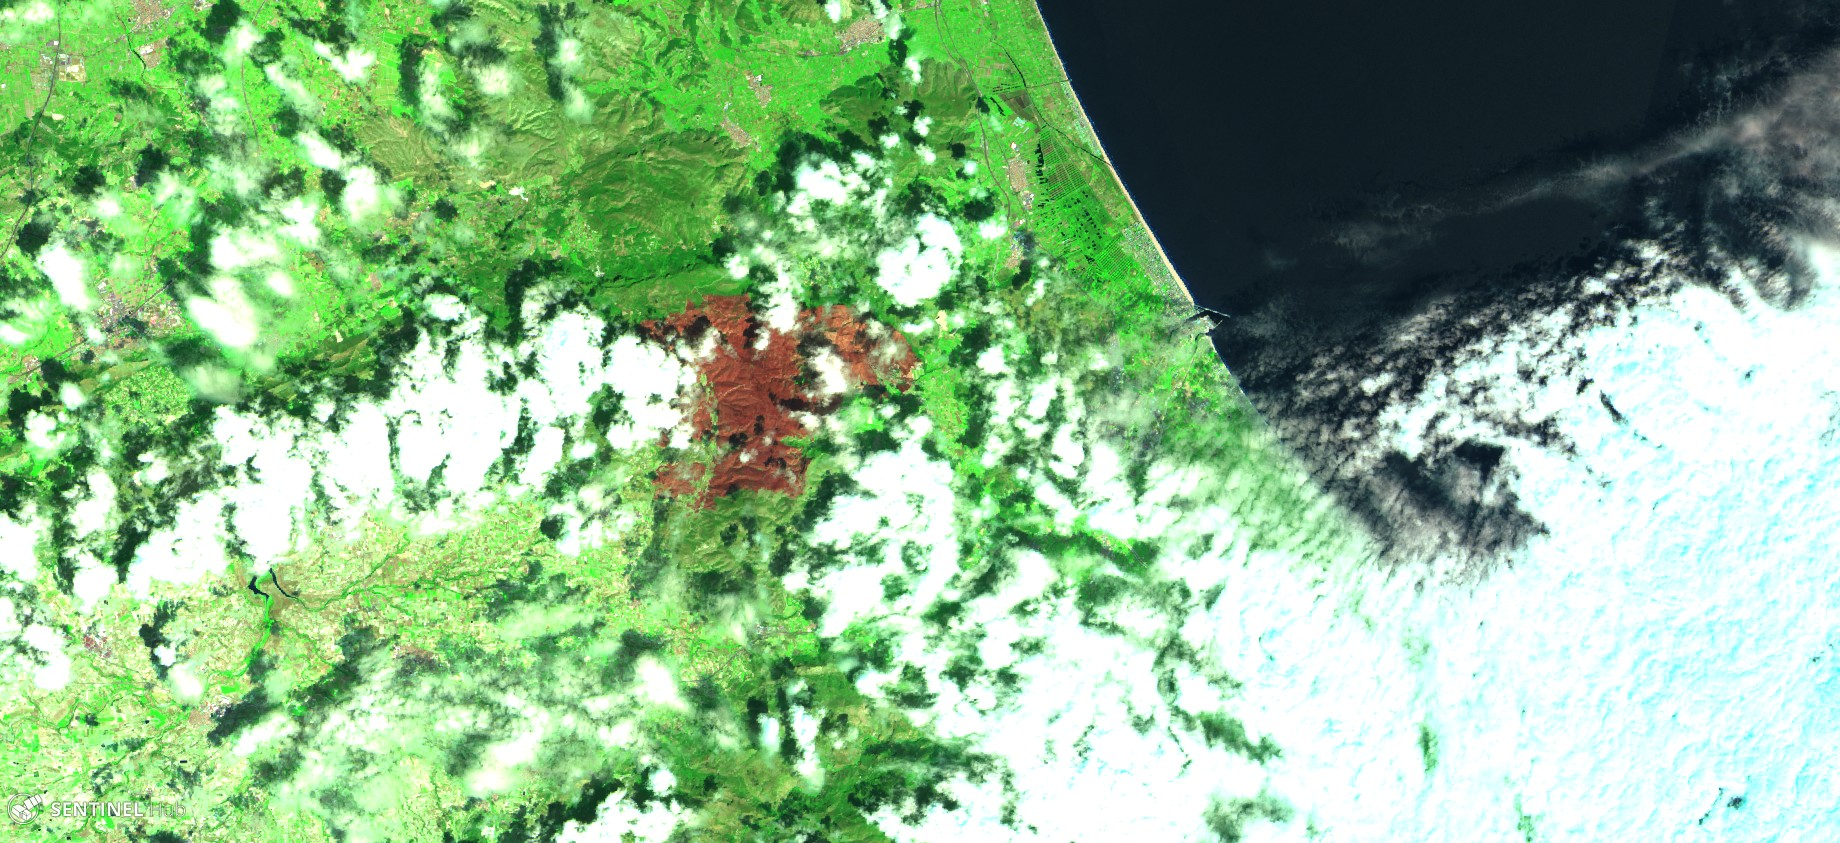
\includegraphics[width=150mm,height=100mm]{figura3}
	\caption{Incendio visto desde satélite Sentinel 2}
	\label{Figura}
\end{figure}

Nullam viverra id risus ut condimentum. Morbi lobortis fermentum vulputate. Duis ut semper mauris. Pellentesque in velit a dui vulputate convallis a eu purus. Integer viverra, nunc vel dignissim pellentesque, urna justo viverra ex, vulputate commodo lorem nibh in sapien. Nunc nec lacinia massa. Maecenas sed suscipit leo. Mauris \cite{Bib02} egestas magna ac pretium condimentum. Phasellus ultricies mi eget odio suscipit ultrices. Cras elementum a turpis ac finibus.

\part{Fórmulas y ecuaciones}
En este apartado encontrareis representadas las formulas utilizadas en  este artículo:\\
\begin{displaymath}
\cos (2\theta) = \cos^2 \theta - \sin^2 \theta
\end{displaymath}\\
\begin{equation}
\frac{
	\begin{array}[b]{r}
	\left( x_1 x_2 \right)\\
	\times \left( x'_1 x'_2 \right)
	\end{array}
}{
	\left( y_1y_2y_3y_4 \right)
}
\end{equation}\\
\begin{displaymath}
\sqrt[n]{1+x+x^2+x^3+\dots+x^n}
\end{displaymath}\\

\part{Bibliografía}
\bibliography{Pedro}
\bibliographystyle{alpha}


\end{document}